\documentclass[UTF8,a4paper]{ctexart}
\usepackage[margin=1in]{geometry}
\usepackage{fancyhdr,hyperref,graphicx,float,subcaption,color}
\pagestyle{fancy}
\hypersetup{hidelinks}

\lhead{\bfseries \leftmark}
\chead{}
\rhead{SCUT}
\lfoot{\url{https://github.com/285571052}}
\cfoot{qhy}
\rfoot{\thepage}
\setlength{\headheight}{13pt}
\renewcommand{\headrulewidth}{0.4pt}
\renewcommand{\footrulewidth}{0.4pt}

\setlength{\parindent}{0pt}
\newcommand{\spaceline}{\vspace{\baselineskip}}

\author{ qhy }
\date{\today}
\title{Dynamic Time Warping(DTW)}

\begin{document}
  \maketitle
  \tableofcontents
  \newpage

  \section{Dynamic Time Warping(DTW)}
  \textbf{如何度量两个等长时间序列之间的距离?}\\
  基本的想法就是使用欧式距离,但是欧式距离有以下缺点:
  欧式距离的局限在于其每个时间点对应的位置是唯一的,
  也就是说,相同的两个时间序列,如果一个时间序列往后挪了小段时刻,
  那么计算出来的欧式距离可能偏差很大。
  \begin{figure}[H]
    \centering
    \begin{subfigure}[H]{0.4\textwidth}
        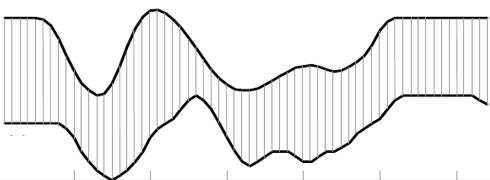
\includegraphics[width=\textwidth]{assets/DynamicTimeWarping(DTW)_bb83b.png}
        \caption{欧式距离}
    \end{subfigure}
    \begin{subfigure}[H]{0.4\textwidth}
        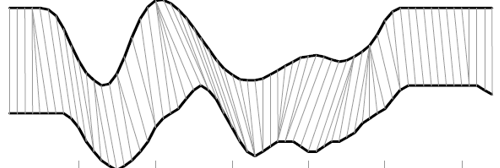
\includegraphics[width=\textwidth]{assets/DynamicTimeWarping(DTW)_5eacd.png}
        \caption{其他}
    \end{subfigure}
    \caption{两个时间序列距离的计算}
  \end{figure}

  对于左图,是普通的欧式距离,但如果采用右图的映射计算方式\footnote{即一个点映射多个点,相应的,另一边的一个点也要映射多个点回去才能平衡}
  ,计算得到值会比欧式距离小得多,也合理得多。

  \spaceline

  \textbf{如何度量两个不等长的时间序列之间的距离?}\\
  想法是把不等长变得等长,简单地说,就是把短的序列变成和长序列等长的序列。

  \spaceline

  对于上述两个问题,可以使用\textbf{DTW}来解决。\\
  首先是不等长的情况,从对应关系的角度来看,只需要短序列的一个点能对应长序列的多个点即可解决问题。\\
  从对应关系的角度来看,序列的点之间的对应关系可能有多重,这里我们取距离最小的一个情况。

  \spaceline

  实际上,这是一个最短路径的动态规划问题。

  那么对于两个序列$Q,C$,$DTW$的定义如下:
  \begin{equation}
    DTW(Q,C) = \min \sum_{k = 1}^{K} w_k
  \end{equation}

  其中,$K$表示路径的长路,$w_k$表示第k步对应的映射关系的平方和。

  要求:$w_1 = d(1,1) , w_K = d(n,m)$

  具体推导公式为:
  \begin{equation}
    g(i,j) = \min  \left \{
    \begin{array}{l}
      g(i - 1,j) + d(i,j)\\
      g(i - 1, j - 1) + d(i , j)\\
      g(i.j - 1) + d(i , j)
    \end{array}
    \right .
  \end{equation}

  \section{另一种DTW}
  那么对于两个序列$Q,C$,$DTW$的定义如下:
  \begin{equation}
    DTW(Q,C) = \min \frac{1}{K} \sqrt{ \sum_{k = 1}^{K} w_k}
  \end{equation}

  这么定义是为了在上面的$DTW$中,DTW更倾向于走对角线的路径,因为路径步骤更短,
  因此,这里进行了归一化处理。

  这个表达式不能直接用动态规划求解,这里采用一个近似算法:
  \begin{equation}
    DTW(Q,C) = \min \frac{1}{K} \sqrt{ \sum_{k = 1}^{K} w_k}\approx \min \frac{1}{n+m-1} \sqrt{ g(n,m)}
  \end{equation}

  则有以下动态规划过程:
  \begin{equation}
    g(i,j) = \min  \left \{
    \begin{array}{l}
      g(i - 1,j) + d(i,j)\\
      g(i - 1, j - 1) + {\color{red} 2}d(i , j)\\
      g(i.j - 1) + d(i , j)
    \end{array}
    \right .
  \end{equation}

  这里对走对角线的操作给与双倍的惩罚($\times 2$),就使得$K = m+n-1$

  \begin{figure}[H]
    \centering
    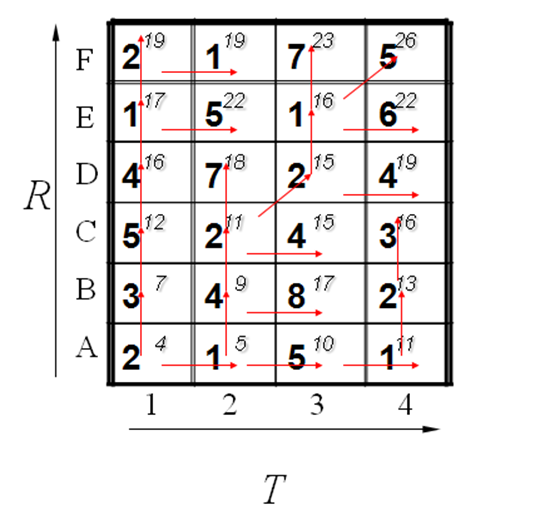
\includegraphics[scale = 0.5]{assets/DynamicTimeWarping(DTW)_6f31e.png}
    \caption{DTW的动态规划过程:初始是从(0,0)开始走,因此(1,1)是$2\times 2 = 4$}
  \end{figure}
  \newpage
  \section{Piecewise Dynamic Time Warping(PDTW)}

  \textbf{Piecewise Aggregate Approximation(PAA):}\\
  每段间隔的数据取均值作为这一段的代表以进行数据的压缩,从而降低计算的开销。

  \begin{figure}[H]
    \centering
    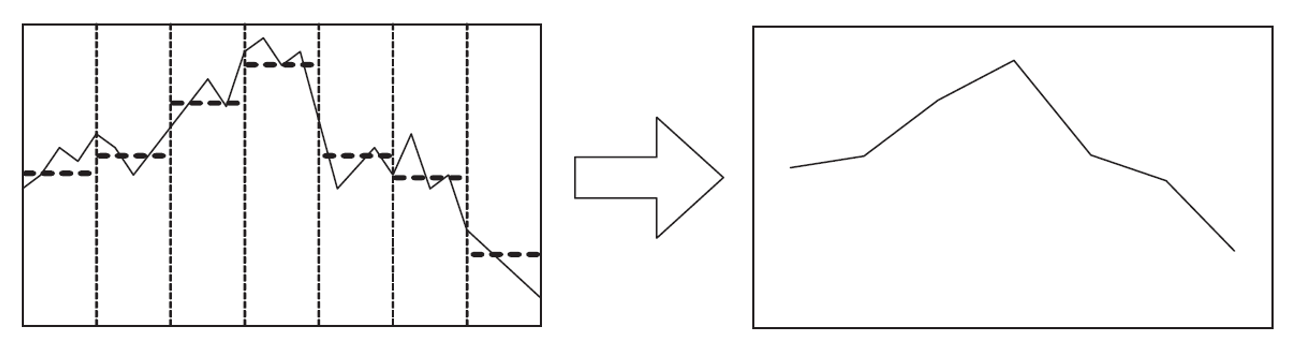
\includegraphics[scale = 0.3]{assets/DynamicTimeWarping(DTW)_1d23a.png}
    \caption{Time series dimensionlity reduction by PAA.The horizontal dotted lines
    show the mean of each segment.}
  \end{figure}

  \spaceline
  \textbf{PDTW = PAA + DTW}
  \begin{figure}[H]
    \centering
    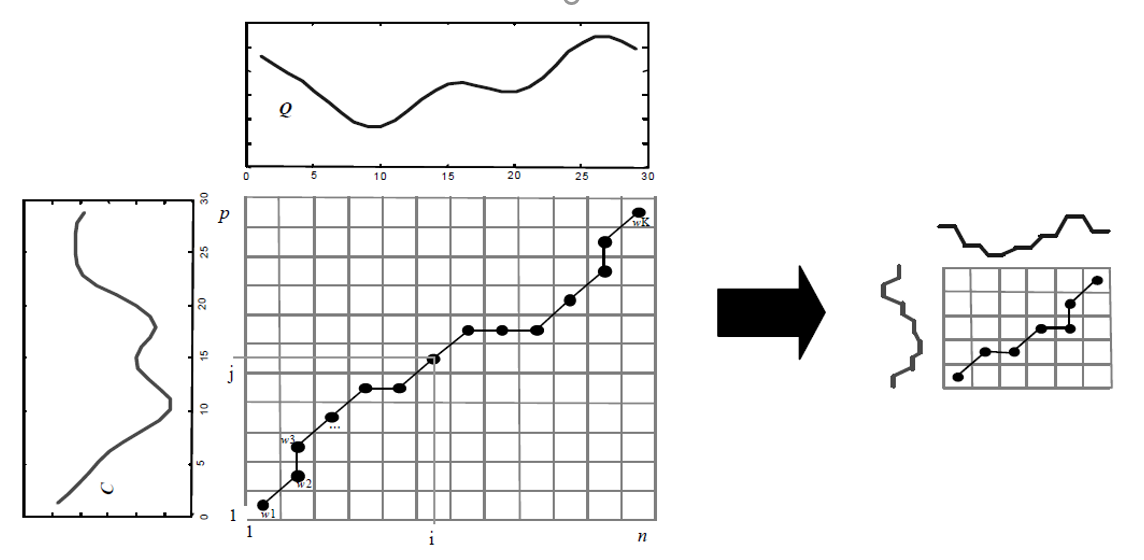
\includegraphics[scale = 0.3]{assets/DynamicTimeWarping(DTW)_35d0b.png}
    \caption{Example of warping path with DTW and PDTW}
  \end{figure}

  注意:$PDTW$虽然减少的计算的开销,但是精度却大大降低了。

  \newpage
  \section{Iterative Deepening DTW(IDDTW 迭代加深DTW)}
  $PDTW$虽然减少了计算的开销,但是却大大减少了精度。

  这里的$IDDTW$虽然还是以$DTW$为名,但更准确地说,应该是在$k-NN$问题中,
  求k近邻的时候,使用迭代加深的思想,提前淘汰不满足要求(距离很大)的时间序列,
  从而避免计算真实$DTW$以减少计算开销。

  $IDDTW$在保持原来计算精度的情况下,使用迭代加深的思想利用$PDTW$
  对一定不满足条件的序列进行提前淘汰,而不用计算到完全的$DTW$,
  从而在保证精度的同时,降低计算的开销。

  注:计算的开销和数据的排列有关,最严重的情况,时间开销会比正常的$DTW$还要多$\frac{1}{3}$

  \spaceline
  \textbf{如何判断一个序列应该被提前淘汰?}
  \begin{figure}[H]
    \centering
    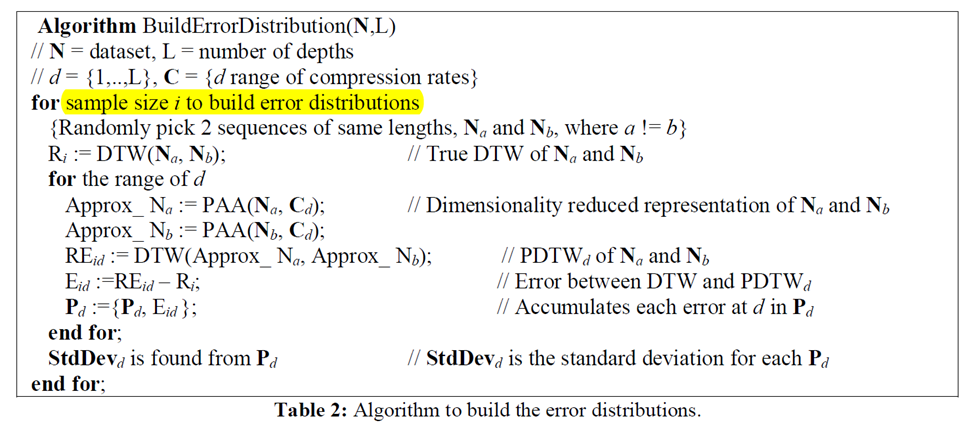
\includegraphics[width = \textwidth]{assets/DynamicTimeWarping(DTW)_58939.png}
  \end{figure}

  在深度为$L$下,我们并不能判断真实的$DTW$是否比当前最好的$DTW$更小,
  这里通过采样的方式,计算在深度$L$的情况下,
  误差的分布(这个分布,用来估计真实的$DTW$与当前深度下的$PDTW$的差距)。

  \spaceline
  那么怎么使用这个分布?

  \begin{figure}[H]
    \centering
    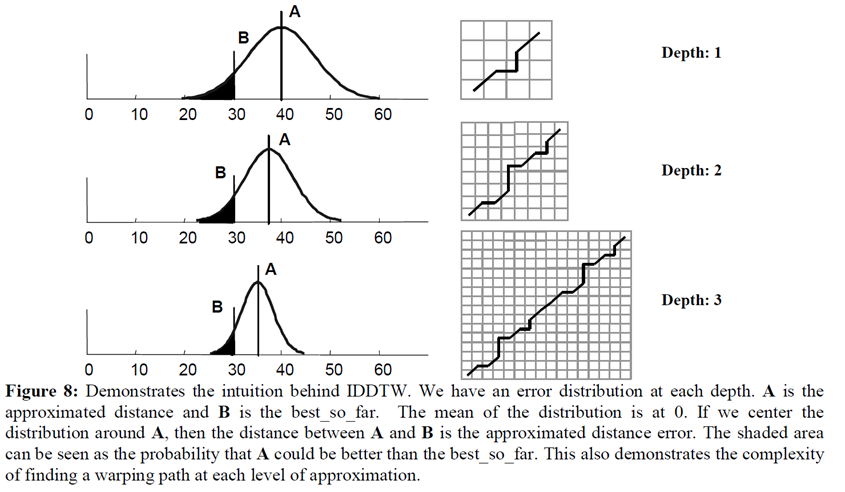
\includegraphics[width = \textwidth]{assets/DynamicTimeWarping(DTW)_026a7.png}
  \end{figure}

  在深度为1的情况下,我们有如图所示的一个分布,$A$表示当前深度下的$DTW$,
  而$B$表示当前最小的 $DTW$ ,这样,黑色的面积就表示当前时间序列,真实的$DTW$
  小于$B$的可能性。

  当这个可能性小于某个阈值的时候,我们就淘汰掉这个时间序列。(如果一个时间序列始终不被淘汰,那么它就会不断加深,
  直到计算出真实的$DTW$)

  上述算法的分布,应该在$k-NN$算法之前预处理出来,而不是$k-NN$过程中计算。

\end{document}
